% Decision tree of insertion sort on three elements (generated by figs_c2ch01.py).
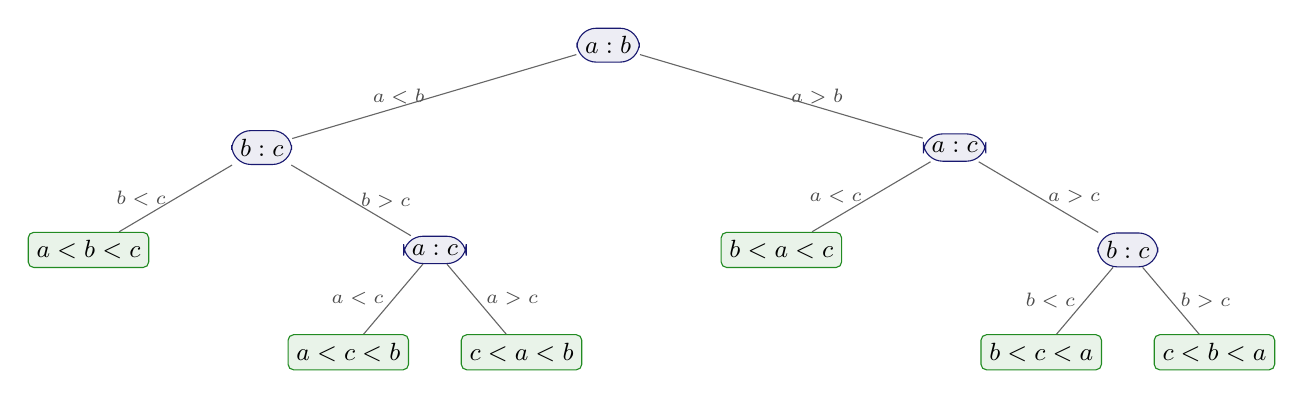
\begin{tikzpicture}[x=1cm,y=1cm,every node/.style={font=\small}]
\tikzset{q/.style={draw=MidnightBlue,fill=MidnightBlue!8,rounded corners=7pt,inner sep=3pt},lf/.style={draw=ForestGreen,fill=ForestGreen!10,rounded corners=2pt,inner sep=3pt}}
\node[q] (t0) at (0.00,0.00) {$a:b$};
\node[q] (t1) at (-4.40,-1.30) {$b:c$};
\draw[black!60] (t0) -- node[left,font=\scriptsize,black!70] {$a<b$} (t1);
\node[lf] (t2) at (-6.60,-2.60) {$a<b<c$};
\draw[black!60] (t1) -- node[left,font=\scriptsize,black!70] {$b<c$} (t2);
\node[q] (t3) at (-2.20,-2.60) {$a:c$};
\draw[black!60] (t1) -- node[right,font=\scriptsize,black!70] {$b>c$} (t3);
\node[lf] (t4) at (-3.30,-3.90) {$a<c<b$};
\draw[black!60] (t3) -- node[left,font=\scriptsize,black!70] {$a<c$} (t4);
\node[lf] (t5) at (-1.10,-3.90) {$c<a<b$};
\draw[black!60] (t3) -- node[right,font=\scriptsize,black!70] {$a>c$} (t5);
\node[q] (t6) at (4.40,-1.30) {$a:c$};
\draw[black!60] (t0) -- node[right,font=\scriptsize,black!70] {$a>b$} (t6);
\node[lf] (t7) at (2.20,-2.60) {$b<a<c$};
\draw[black!60] (t6) -- node[left,font=\scriptsize,black!70] {$a<c$} (t7);
\node[q] (t8) at (6.60,-2.60) {$b:c$};
\draw[black!60] (t6) -- node[right,font=\scriptsize,black!70] {$a>c$} (t8);
\node[lf] (t9) at (5.50,-3.90) {$b<c<a$};
\draw[black!60] (t8) -- node[left,font=\scriptsize,black!70] {$b<c$} (t9);
\node[lf] (t10) at (7.70,-3.90) {$c<b<a$};
\draw[black!60] (t8) -- node[right,font=\scriptsize,black!70] {$b>c$} (t10);
\end{tikzpicture}
